\documentclass[11pt]{article}
% AutoLabs Experiment 3C. Numerical results retain the recorded run values.
\usepackage[margin=1in]{geometry}
\usepackage{amsmath,amssymb,booktabs,graphicx}
\usepackage{pgfplots}
\pgfplotsset{compat=1.17}
\usepackage[hidelinks]{hyperref}
\usepackage{titlesec}
\usepackage[numbers]{natbib}
\titlespacing*{\section}{0pt}{1.1em}{0.5em}
\title{\textbf{Evaluating Unsupervised Discovery of Persona-Relevant Directions\\with Matryoshka Sparse Autoencoders}}
\author{Raphael Khalid \\ \small AutoLabs \\ \small \texttt{autolabs-ebon.vercel.app}}
\date{September 2026 (working paper)}
\setlength{\emergencystretch}{3em}
\begin{document}
\maketitle

\begin{abstract}
Can sparse autoencoders identify persona-relevant directions without a
prespecified target trait? I investigate this question using a Matryoshka
BatchTopK sparse autoencoder trained on $100$M assistant-position tokens from
\texttt{Qwen2.5-7B-Instruct}. The autoencoder has approximately $235$M parameters
and $32{,}768$ features at decoder layer $19$, with held-out fraction of variance
explained $0.717$ and mean $L_0=40$. Candidate selection comprises an
assistant-specificity arm, a firing-density comparison arm, and a prompt-informed
comparison arm. Across $24$ scenarios, $60$ of $128$ features satisfy a diagnostic
criterion combining residual separability and cross-scenario consistency; two of
three supervised persona-vector controls also satisfy it. A blinded language-model
judge produces consistent speaker-related descriptions for $10$ signed directions,
representing $9$ distinct features. All $10$ also satisfy the screening criterion.
Two originate from selection without persona prompts and eight from
prompt-informed selection. However, inspection of the two prompt-free candidates
reveals substantial confounding by output degradation. One produces only
punctuation in all $24$ scenarios, with the judge attributing the named property
to the baseline response; the other frequently fails the coherence proxy.
The study therefore identifies behaviour-changing candidates but does not yet
establish coherent persona discovery without target-trait specification. It
provides an empirical evaluation of the discovery question raised by
\citet{chen2025persona} and identifies limitations of the screening and naming
criteria. Prompt reachability was omitted from the final run; the ease of prompt
elicitation remains a question for future work.
\end{abstract}

\section{Introduction}
Persona vectors represent behavioural traits as directions in a language model's
activation space. The extraction method of \citet{chen2025persona} begins with a
specified trait and uses contrasting prompted responses to estimate its direction.
Their limitations section identifies dependence on advance trait specification,
an adequate natural-language description, and successful prompt elicitation. It
proposes sparse autoencoders (SAEs) as a complementary route to discovering
persona-relevant directions.

Experiment 3C examines discovery before trait naming. I train an SAE to
reconstruct residual-stream activations, select candidate features, intervene
along their decoder directions, and obtain descriptions from blinded comparisons
of generated responses. The central question is whether this process can identify
coherent persona-relevant changes without a target trait serving as the
candidate-selection criterion.

Dictionary learning and candidate selection require separate interpretation.
The entire SAE dictionary is learned without trait labels. One selection arm,
however, uses manually specified persona prompts. Evidence for discovery without
persona prompts must therefore come from the other arms. I use
\emph{persona-relevant} for effects concerning voice, stance, self-presentation,
or relation to the reader. Such a description does not by itself establish a
complete persona, a distinct psychological category, or a selective intervention.

\section{Background and contribution}
BatchTopK SAEs constrain the number of active features across a batch while
allowing sparsity to vary between tokens \citep{bussmann2024batchtopk}.
Matryoshka SAEs train nested dictionary prefixes to reconstruct the same
activations, encouraging representations at multiple levels of granularity
\citep{bussmann2025matryoshka}. I combine these methods to construct the feature
dictionary used here.

Appendix M of \citet{chen2025persona} already examines SAE features selected by
alignment with specified persona vectors. The present study evaluates selection
without that trait-specific alignment, alongside density-based and prompt-informed
comparisons. Random directions and supervised persona vectors provide reference
measurements. Blinded descriptions assess whether changes concern the speaker.
The contribution is this experimental evaluation and the accompanying analysis
of its failure modes, rather than a claim to have established unlabelled persona
discovery or priority over all other discovery methods.

\section{Methods}
\subsection{Model, data, and autoencoder}
The base model is \texttt{Qwen2.5-7B-Instruct}. Activations are collected at the
output of decoder layer $19$ using zero-based indexing. The SAE contains
approximately $235$M parameters and nested dictionary widths of $1{,}024$,
$4{,}096$, $16{,}384$, and $32{,}768$. BatchTopK uses $k=40$, specifying average
batch sparsity rather than exactly $40$ active features at every token.

Training uses $100$M assistant-position tokens. The configured mixture draws
conversations from LMSYS-Chat-1M, \texttt{monology/pile-uncopyrighted}, and an
insecure-code dataset with sampling weights $0.70$, $0.22$, and $0.08$,
respectively. These are conversation-sampling weights, not measured token
fractions. Plain-text samples are placed in assistant turns. Downstream screens
reuse the trained checkpoint rather than training a new SAE for each screen.

\subsection{Candidate selection}
The final screen contains $128$ distinct features in three disjoint arms:
\begin{itemize}
\item \textbf{Assistant-specificity ($48$ features).} Selection uses
assistant-versus-user activation statistics, breadth across conversations,
topic-invariance proxies, and dictionary structure, without persona prompts or
a trait-specific target description.
\item \textbf{Density-quantile ($32$ features).} Features are sampled across
firing-density quantiles as a comparison that also does not use persona prompts.
\item \textbf{Prompt-shift ($48$ features).} Selection uses activation variation
across manually specified persona-style contexts. This arm is prompt-informed
and does not independently test discovery without persona prompts.
\end{itemize}
The assistant-specificity arm depends on researcher-designed ranking heuristics;
absence of trait labels does not imply absence of inductive bias.

\subsection{Steering and controls}
Both signs of each feature are evaluated. Calibration tests doses of $0.25$,
$0.5$, $1.0$, and $2.0$ relative to its recorded maximum activation. A dose is
accepted when at least $75\%$ of calibration scenarios pass the coherence proxy;
the largest accepted dose is selected, with a fallback when none qualifies.
The final screen compares steered and baseline responses across $24$ scenarios.
Calibration does not guarantee coherent output on the screening scenarios.

Three supervised control vectors are constructed from differences in mean
activations under contrasting prompts: evil versus benevolent, sycophantic versus
honest, and hallucinating versus factual. These implement a contrastive
comparison, not a complete replication of the original persona-vector evaluation.
The screen also includes $20$ random directions. Random directions use normalized
Gaussian vectors scaled by a nominal dose; feature interventions additionally
scale by the feature's maximum activation. Their perturbation norms are therefore
not matched, limiting the interpretation of the random comparison.

\subsection{Diagnostic screening}
Leave-one-scenario-out logistic regression measures separability of steered and
baseline responses in mean residual and hashed lexical representations. The
criterion $G_0$ uses only residual-view AUC. For signed direction $d$, let $A_d$
denote this AUC, $C_d$ the mean pairwise cosine similarity between its
scenario-specific response differences, and $N_d$ a reference similarity to
differences sampled from other directions. The criterion is
\[
G_0(d)=\mathbf{1}\!\left[A_d>\max_{r\in\mathcal R}A_r
\quad\text{and}\quad C_d-N_d>0.1\right],
\]
where $\mathcal R$ contains the $20$ random directions. The consistency reference
includes other feature, control, and random directions, rather than random
directions alone. A feature or control passes if either sign passes. Lexical AUC
is supplementary and is not part of $G_0$.

The implementation reports $G_0$ diagnostically. It does not automatically block
judge evaluation when candidates or controls fail. Control pass counts are
therefore reference results rather than certification of the discovery method.

\subsection{Blinded description and naming}
Judge evaluation selects the $40$ highest-ranked signed directions by residual
AUC, with consistency as a tie-breaker, and adds the three random directions with
the lowest residual AUC. Selection does not require $G_0$ passage. Each
steered-baseline pair is presented in both orders. The judge,
\texttt{gpt-5.6-luna}, identifies a distinguishing property and classifies it as
speaker-, content-, or format-related, or reports no distinction. Feature
identities and intervention conditions are withheld from the comparison.

Descriptions are clustered using sentence embeddings and a keyword-overlap merge
step. A direction is named when the largest cluster contains at least half of the
non-null descriptions, at least $80\%$ of that cluster agrees on which response
expresses the property more, and a strict majority is speaker-related. If $q_d$
is the largest cluster's fraction of non-null descriptions and $a_d$ its polarity
agreement, the naming score is $S_d=q_da_d$. The above-null criterion requires
$S_d$ to exceed the highest score of the three judged random directions by $0.1$.
This is an empirical threshold, not a calibrated significance test.

The naming rule accepts either polarity. A label may describe a property of the
baseline response that is absent after steering. The two orderings of each pair
are repeated assessments, not independent scenarios. These distinctions are
necessary when interpreting the resulting labels.

\subsection{Completed scope}
Training, ranking, calibration, screening, and blinded description were completed.
Prompt reachability was deliberately omitted from the final run. Existing
reach-probe code and earlier pilot artifacts do not constitute a final-run
reachability result. I reserve prompt-elicitation difficulty for future work.

\section{Results}
\subsection{Reconstruction quality}
Held-out fraction of variance explained is $0.717$, with mean $L_0=40.0$
(Table~\ref{tab:sae}). Training-batch FVE approaches $0.75$
(Figure~\ref{fig:train}); this is distinct from the held-out estimate. The saved
reconstruction-replacement check records next-token argmax agreement of $0.780$
over $118$ assistant positions, below its configured $0.90$ threshold. The check
therefore fails. Decoder-direction steering does not itself replace the residual
stream with the SAE reconstruction, but the failed check limits fidelity claims.

\begin{table}[htbp]\centering
\begin{tabular}{lc}
\toprule
Measure & Recorded value \\
\midrule
Held-out FVE & $0.717$ \\
Held-out mean $L_0$ & $40.0$ \\
Replacement-check argmax agreement & $0.780$ \\
Replacement-check cross-entropy increase & $0.566$ nats \\
Replacement-check acceptance threshold & $0.90$ (not met) \\
\bottomrule
\end{tabular}
\caption{Saved post-training diagnostics for the checkpoint used in the final screen.}
\label{tab:sae}
\end{table}

\begin{figure}[htbp]\centering
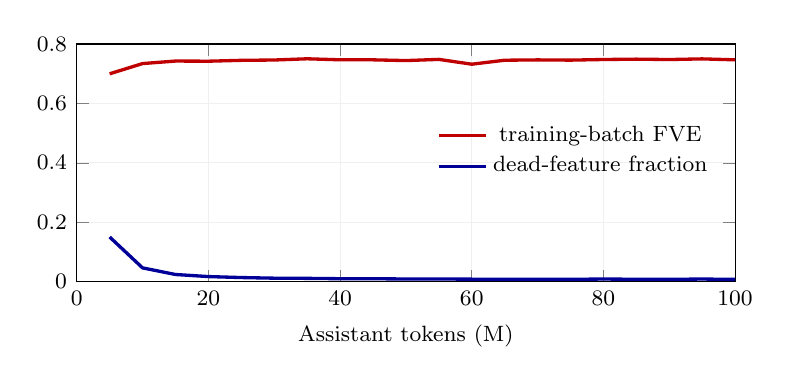
\begin{tikzpicture}
\begin{axis}[width=0.82\linewidth,height=4.6cm,xlabel={Assistant tokens (M)},
xmin=0,xmax=100,ymin=0,ymax=0.8,
legend style={at={(0.98,0.55)},anchor=east,font=\footnotesize,draw=none,fill=none},
grid=both,grid style={gray!12},tick label style={font=\footnotesize},
label style={font=\footnotesize}]
\addplot[color=red!75!black,very thick,mark=none] coordinates {
(5.0,0.6998) (10.0,0.7342) (15.0,0.7427) (20.0,0.7422) (25.0,0.7451)
(30.0,0.7462) (35.0,0.7503) (40.0,0.7469) (45.0,0.7468) (50.0,0.7443)
(55.0,0.7483) (60.0,0.7321) (65.0,0.7455) (70.0,0.7466) (75.0,0.7458)
(80.0,0.7479) (85.0,0.7491) (90.0,0.7478) (95.0,0.7500) (100.0,0.7468)};
\addlegendentry{training-batch FVE}
\addplot[color=blue!60!black,very thick,mark=none] coordinates {
(5.0,0.1504) (10.0,0.0464) (15.0,0.0242) (20.0,0.0172) (25.0,0.0139)
(30.0,0.0118) (35.0,0.0112) (40.0,0.0100) (45.0,0.0099) (50.0,0.0091)
(55.0,0.0090) (60.0,0.0085) (65.0,0.0083) (70.0,0.0082) (75.0,0.0080)
(80.0,0.0089) (85.0,0.0082) (90.0,0.0079) (95.0,0.0089) (100.0,0.0077)};
\addlegendentry{dead-feature fraction}
\end{axis}
\end{tikzpicture}
\caption{Recorded training diagnostics from run \texttt{persona-3c-d77e7c1e}.
These checkpoint values are training-batch measurements, not repeated held-out
evaluations or independent replications.}
\label{fig:train}
\end{figure}

\subsection{Screening outcomes}
An earlier eight-scenario screen records $96/256$ features passing $G_0$ while
one of its three controls passes. The final $24$-scenario screen records
$60/128$ features passing in at least one sign, or $79/256$ signed directions.
The sycophantic and hallucinating controls pass; the evil control does not.
This provides positive-control support for two contrasts without establishing
sensitivity to all persona-related effects.

The screens differ in candidate count and other settings. Their comparison does
not isolate the effect of scenario count, and no formal power analysis is
reported. The failed control does not establish that feature counts are
conservative or identify why that control failed.

\begin{table}[htbp]\centering\small
\begin{tabular}{lrrrr}
\toprule
Selection arm & Features & $G_0$ features & Judged signs & Named signs \\
\midrule
Assistant-specificity & 48 & 25 & 17 & 2 \\
Density-quantile & 32 & 10 & 5 & 0 \\
Prompt-shift & 48 & 25 & 18 & 8 \\
\midrule
Total & 128 & 60 & 40 & 10 \\
\bottomrule
\end{tabular}
\caption{Final screening and naming outcomes. Feature counts group both signs;
judge and naming counts refer to signed directions. Unequal, selective judge
coverage prevents interpreting naming totals as comparable discovery rates.}
\label{tab:arms}
\end{table}

\subsection{Named directions and output quality}
The saved judge output contains $2{,}063$ responses from $2{,}064$ planned
comparisons. Each selected feature direction has $48$ responses; one random
direction has $47$. The maximum null naming score is $0.175$, yielding an
above-null threshold of $0.275$. Ten signed feature directions meet the naming
criteria and also pass $G_0$ (Table~\ref{tab:named}). They correspond to nine
features because both signs of feature $2036$ are named. Several descriptions
also overlap semantically. The count does not establish ten distinct personas.

\begin{table}[htbp]\centering\small
\begin{tabular}{rllrr}
\toprule
Feature/sign & Arm & Judge-derived description & Cluster & Agreement \\
\midrule
$148+$ & A & engaged and supportive & $36/48$ & $1.00$ \\
$717+$ & A & composed and confident & $26/48$ & $0.96$ \\
$89-$ & P & more empathetic and conversational & $34/48$ & $0.97$ \\
$241-$ & P & formal, academic tone & $27/48$ & $1.00$ \\
$362-$ & P & empathetic and personally supportive & $26/48$ & $1.00$ \\
$586+$ & P & enthusiastic and personally affirming & $34/48$ & $0.97$ \\
$709+$ & P & playful, humorous tone & $42/48$ & $0.95$ \\
$931+$ & P & formal and self-explanatory & $24/48$ & $0.96$ \\
$2036+$ & P & formal, academic tone & $26/48$ & $0.88$ \\
$2036-$ & P & friendly, conversational warmth & $33/48$ & $1.00$ \\
\bottomrule
\end{tabular}
\caption{All ten named signed candidates. A: assistant-specificity; P:
prompt-shift. Cluster is the largest semantic cluster among non-null descriptions.
Agreement is polarity agreement within that cluster, not agreement across all
judgements. A label can describe the baseline rather than the steered response.}
\label{tab:named}
\end{table}

The two assistant-specificity candidates require particular scrutiny. Feature
$148+$ produces a single full stop in $23$ scenarios and four full stops in the
remaining scenario. All $48$ judge comparisons attribute the distinguishing
property more strongly to the baseline. Its label therefore describes a contrast
with collapsed output, not an induced supportive persona. The coherence proxy
nevertheless accepts $23/24$ responses because it lacks a minimum substantive
response requirement. That high proxy score is not evidence of usable output.

Feature $717+$ passes the coherence proxy on only $8/24$ scenarios. Its recorded
responses exhibit substantial degradation, and the confidence-related label does
not establish selective control of confidence. These observations prevent
interpreting the two prompt-free named candidates as clean demonstrations of
unlabelled persona discovery. The remaining eight named directions originate from
prompt-informed selection and require separate quality assessment; they do not
resolve the prompt-free claim.

\section{Discussion and limitations}
Experiment 3C completed the planned discovery and description stages and
identified reproducible records of behaviour-changing interventions. However,
the central scientific claim requires more than separability and a consistent
speaker-related label. Output collapse can satisfy both criteria when the judge
consistently describes qualities retained by the baseline. This failure mode is
present in the strongest-scoring prompt-free candidate.

The result therefore provides an informative test of SAE-based discovery, but
not sufficient evidence that coherent unlabelled personas were discovered.
Successful execution of the pipeline and passage of its numerical criteria should
be distinguished from validation of the intended construct. Future evaluation
should require substantive, coherent responses and assess semantic specificity
while explicitly preserving the direction of each judged contrast.

Additional limitations include one model, one layer, one training configuration,
and no independent seed replications. Naming relies on one language-model judge
and post hoc clustering without independent human validation. The three naming
nulls are selected for low residual AUC, whereas evaluated features are selected
for high AUC; screening perturbation norms are also unmatched. Finite null maxima
and fixed margins do not provide a calibrated false-discovery rate across the
searched dictionary. Unequal judge coverage further limits comparisons between
selection arms. Leave-one-scenario-out prediction does not turn exploratory
method development into an independent confirmatory test.

Prompt reachability is a separate question. Direct activation intervention neither
proves nor disproves that prompting can reproduce a behavioural effect. I did not
evaluate reachability in the final run. Future work should measure prompt-search
attempts, prompt length, and achievable effect size under explicit budgets,
matched output quality, and held-out scenarios. This would address ease of
elicitation after coherent candidate effects have been established.

\section{Conclusion}
The trained SAE and completed screening pipeline identify ten named signed
candidates across nine features. Two are selected without persona prompts, but
inspection reveals output collapse or degradation that confounds their
interpretation. The current evidence therefore does not establish coherent
unlabelled persona discovery. It extends the empirical investigation proposed by
\citet{chen2025persona} by evaluating a discovery procedure and identifying
necessary improvements to its validity checks. The ease of prompt elicitation
remains outside the completed study.

\section*{Artifacts and authorship}
The training run is \texttt{persona-3c-d77e7c1e}; the final screen is
\texttt{persona-3c-ded5477e-\allowbreak{}a5c3-\allowbreak{}4372-\allowbreak{}a776-\allowbreak{}91a0357293e1}.
Code, configurations, and publication sources are available in the
\href{https://github.com/RaphaelKhalid/autolabs/tree/main/research/experiment-003c}{AutoLabs repository}.
The checkpoint is hosted at
\href{https://huggingface.co/RaphaelRaphaelRaphael/autolabs-3c-sae}{Hugging Face}.
Results are derived from the saved \texttt{screen\_records.json},
\texttt{screen\_generations.json}, \texttt{describe\_results.json}, and
\texttt{post\_train\_check.json} outputs. Raphael Khalid is the sole researcher
and author.

\bibliographystyle{plain}
\begin{thebibliography}{3}
\bibitem[Chen et al.(2025)]{chen2025persona}
R.~Chen, A.~Arditi, H.~Sleight, O.~Evans, and J.~Lindsey.
\newblock Persona Vectors: Monitoring and Controlling Character Traits in Language Models.
\newblock \emph{arXiv:2507.21509}, 2025.
\newblock \url{https://arxiv.org/abs/2507.21509}.
\bibitem[Bussmann et al.(2024)]{bussmann2024batchtopk}
B.~Bussmann, P.~Leask, and N.~Nanda.
\newblock BatchTopK Sparse Autoencoders.
\newblock \emph{arXiv:2412.06410}, 2024.
\newblock \url{https://arxiv.org/abs/2412.06410}.
\bibitem[Bussmann et al.(2025)]{bussmann2025matryoshka}
B.~Bussmann, N.~Nabeshima, A.~Karvonen, and N.~Nanda.
\newblock Learning Multi-Level Features with Matryoshka Sparse Autoencoders.
\newblock \emph{Proceedings of the 42nd International Conference on Machine Learning},
267:6077--6101, 2025.
\newblock \url{https://proceedings.mlr.press/v267/bussmann25a.html}.
\end{thebibliography}
\end{document}
